% Implementation chart of the severity-score comparator arm (R/09c_apache.R,
% R/09d_sofa.R, R/10b_severity.R), in the format of the engine chart. Drawn
% 2026-09-25 from docs/figs/callgraph/severity.md: the boxes from its
% reachable-function table, the arrows from its call edges and its table of
% targets and entry-script statements. Redrawn the same day after the arrow
% check was added to the checker; every arrow here is backed by a row of
% those tables except the two `ex` arrows, which cross the process boundary
% (the bundle written by the training run and read by the apply runners).
% `python docs/figs/callgraph_check.py severity` holds this chart to the
% parser-based call graph. Engine boxes are referred to by number (E 5.6 is
% box 5.6 of pipeline_implementation.tex).
%
% Build:  pdflatex pipeline_severity.tex   (from this directory)
\documentclass[10pt]{article}
\usepackage[paperwidth=44cm,paperheight=42cm,margin=8mm]{geometry}
\usepackage[T1]{fontenc}
\usepackage{lmodern}
\usepackage{amsmath}
\usepackage{tikz}
\usetikzlibrary{arrows.meta,fit,backgrounds,calc,positioning}
\pagestyle{empty}
\begin{document}
\centering
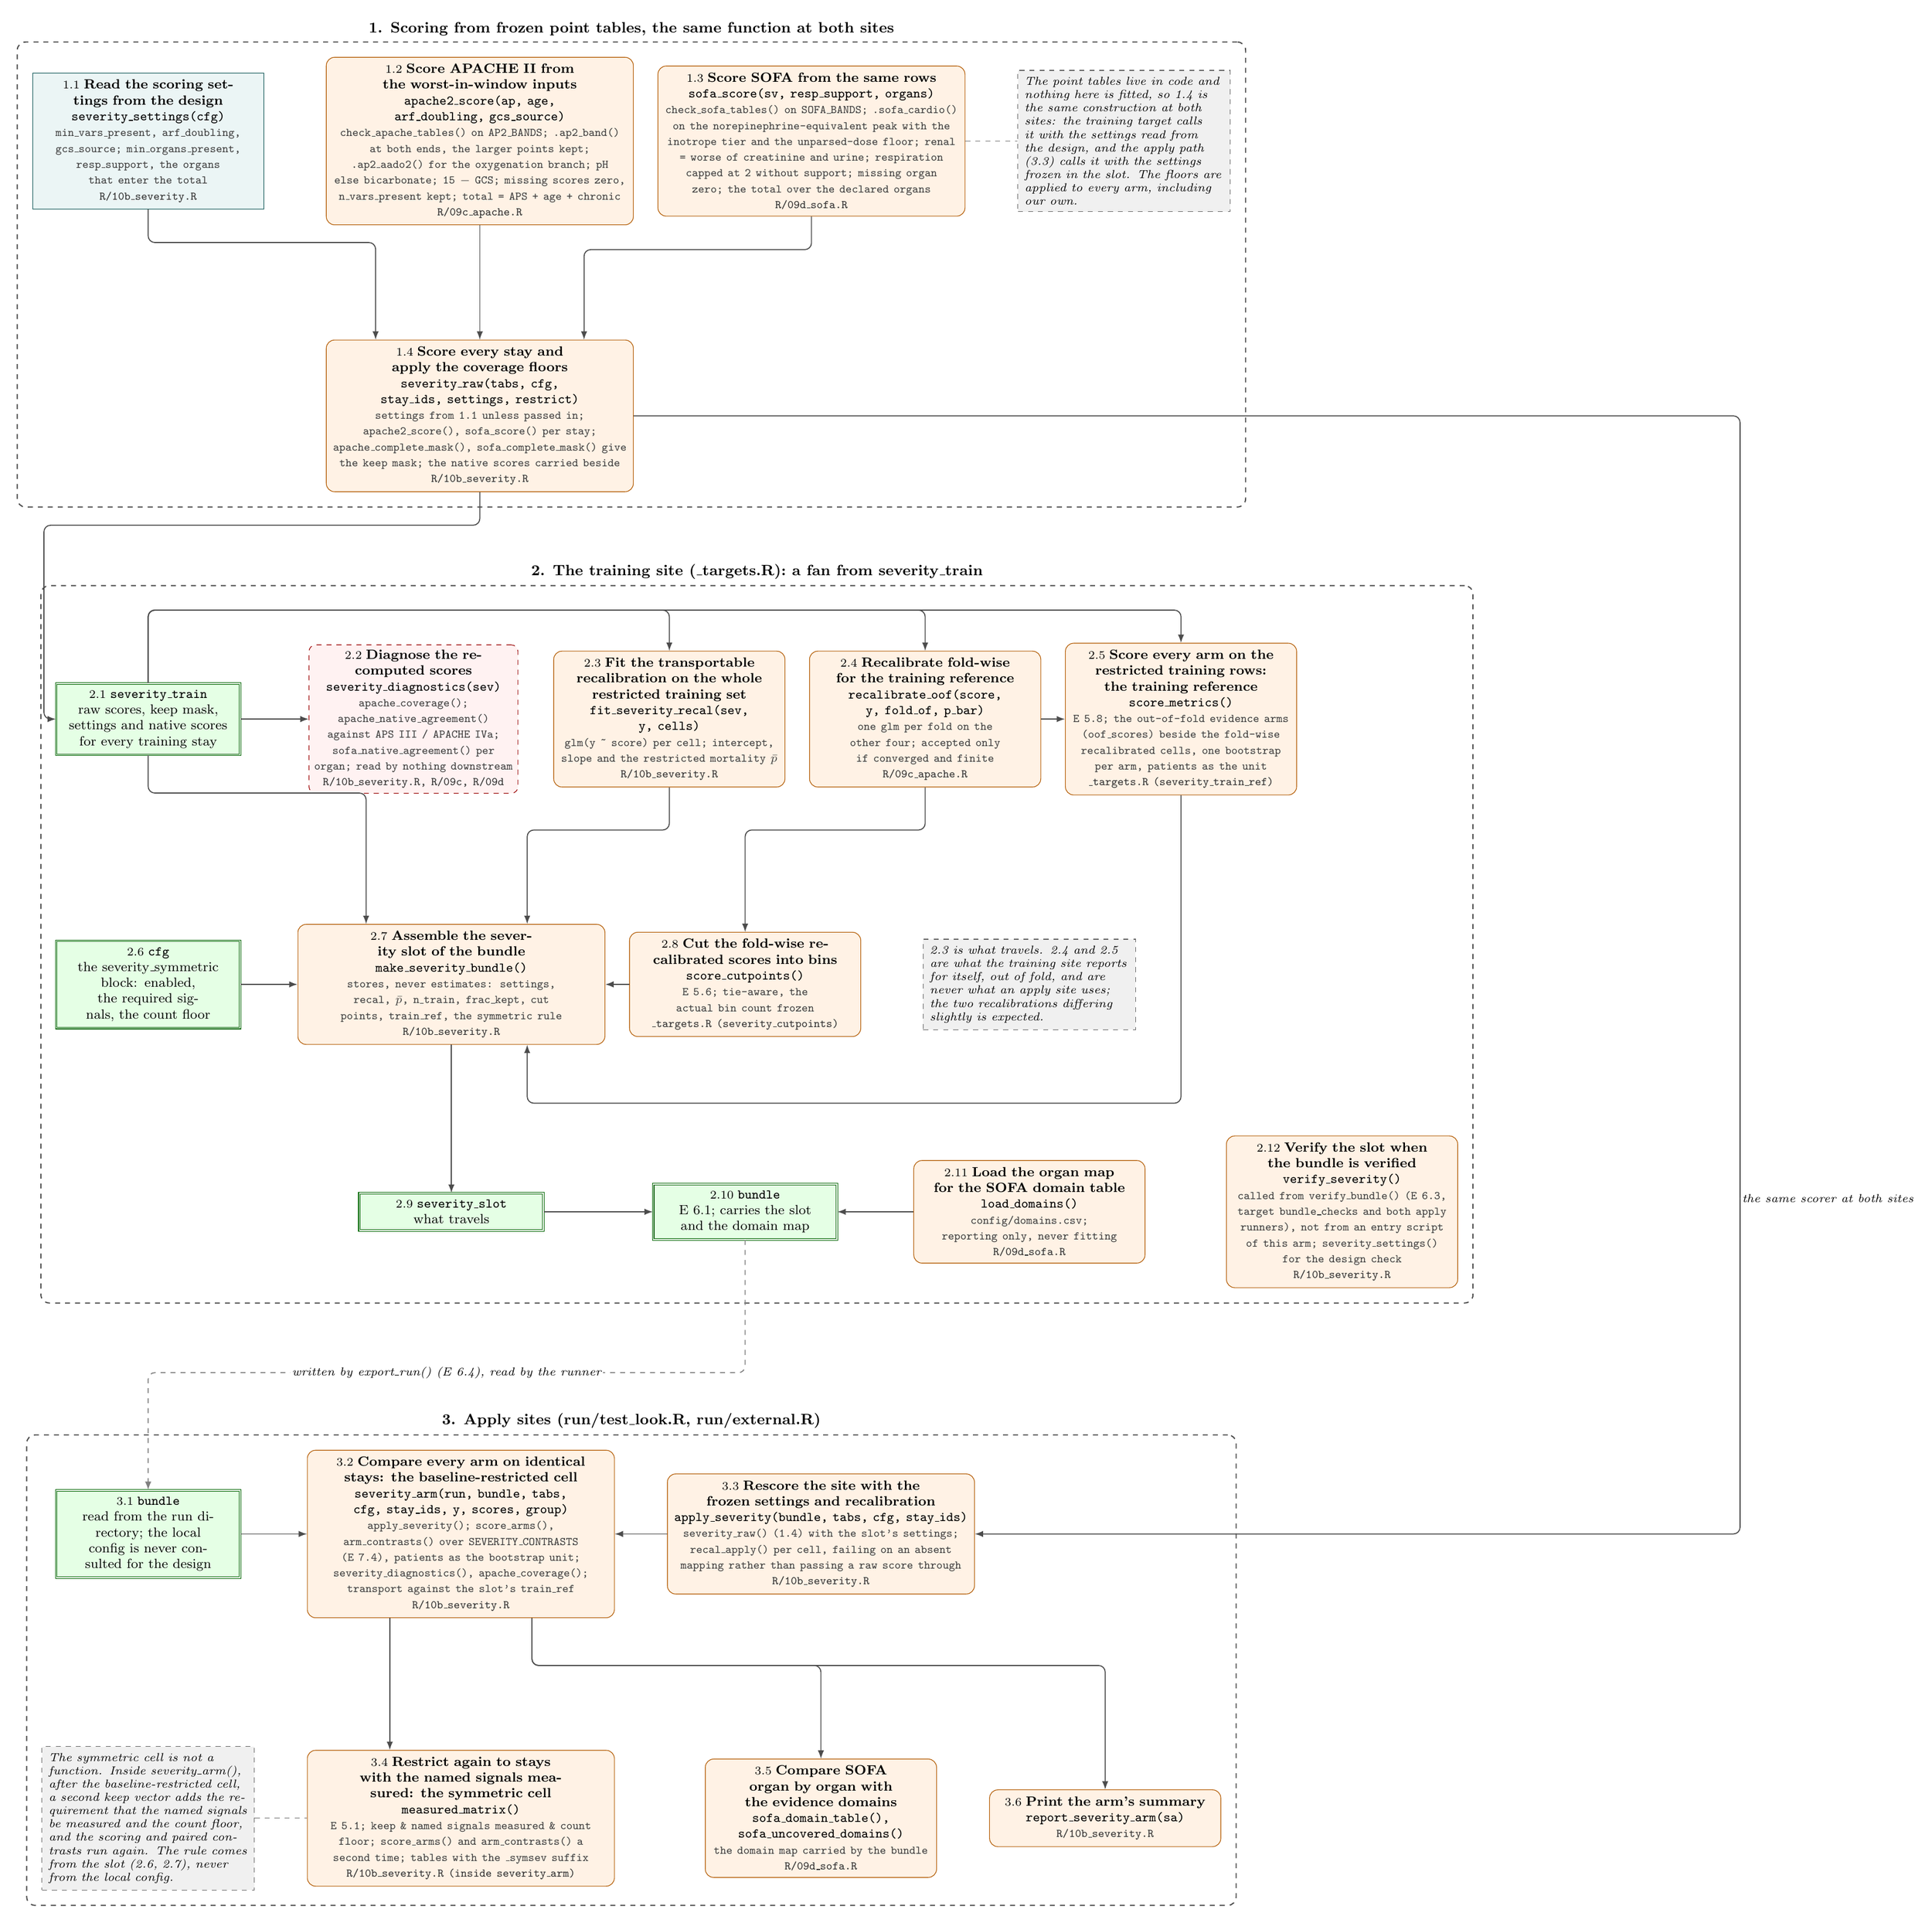
\begin{tikzpicture}[
  font=\footnotesize, x=1cm, y=1cm,
  fn/.style={draw=orange!70!black, fill=orange!10, rounded corners=5pt, align=center, inner sep=4pt, text width=4.6cm},
  fnw/.style={fn, text width=6.2cm},
  obj/.style={draw=blue!50!black!60, fill=blue!8, rounded corners=2pt, align=center, inner sep=4pt, text width=3.4cm},
  chk/.style={draw=red!60!black, fill=red!5, dashed, rounded corners=4pt, align=center, inner sep=3pt, text width=4.2cm},
  dcl/.style={draw=teal!60!black, fill=teal!8, align=center, inner sep=4pt, text width=4.6cm},
  outp/.style={draw=green!40!black, fill=green!10, double, align=center, inner sep=4pt, text width=3.6cm},
  note/.style={draw=black!60, dashed, fill=black!6, align=left, inner sep=4pt, text width=4.2cm, font=\scriptsize\itshape},
  e/.style={-{Latex[length=5pt]}, line width=0.6pt, draw=black!70, rounded corners=4pt},
  ex/.style={e, dashed, draw=black!50},
  en/.style={draw=black!55, dashed, line width=0.4pt},
  grp/.style={draw=black!70, dashed, line width=0.7pt, inner sep=9pt, rounded corners=5pt},
  lab/.style={font=\small\bfseries, anchor=south},
  al/.style={font=\scriptsize\itshape, fill=white, inner sep=1pt}]

\newcommand{\B}[5]{{\scriptsize #1}\;\textbf{#2}\\\texttt{\textbf{#3}}\\{\scriptsize\ttfamily\color{black!75}#4}\\{\scriptsize\ttfamily\color{black!80}#5}}
\newcommand{\Bs}[4]{{\scriptsize #1}\;\textbf{#2}\\\texttt{\textbf{#3}}\\{\scriptsize\ttfamily\color{black!80}#4}}
\newcommand{\Obj}[3]{{\scriptsize #1}\;\texttt{\textbf{#2}}\\#3}

% =====================================================================
% STAGE 1: scoring from frozen point tables, the same function at both sites
% =====================================================================
\node[dcl] (set) at (3.0,0) {\B{1.1}{Read the scoring settings from the design}{severity\_settings(cfg)}{min\_vars\_present, arf\_doubling, gcs\_source; min\_organs\_present, resp\_support, the organs that enter the total}{R/10b\_severity.R}};
\node[fnw] (ap2) at (10.0,0) {\B{1.2}{Score APACHE II from the worst-in-window inputs}{apache2\_score(ap, age, arf\_doubling, gcs\_source)}{check\_apache\_tables() on AP2\_BANDS; .ap2\_band() at both ends, the larger points kept; .ap2\_aado2() for the oxygenation branch; pH else bicarbonate; 15 $-$ GCS; missing scores zero, n\_vars\_present kept; total = APS + age + chronic}{R/09c\_apache.R}};
\node[fnw] (sofa) at (17.0,0) {\B{1.3}{Score SOFA from the same rows}{sofa\_score(sv, resp\_support, organs)}{check\_sofa\_tables() on SOFA\_BANDS; .sofa\_cardio() on the norepinephrine-equivalent peak with the inotrope tier and the unparsed-dose floor; renal = worse of creatinine and urine; respiration capped at 2 without support; missing organ zero; the total over the declared organs}{R/09d\_sofa.R}};
\node[note] (n1) at (23.6,0) {The point tables live in code and nothing here is fitted, so 1.4 is the same construction at both sites: the training target calls it with the settings read from the design, and the apply path (3.3) calls it with the settings frozen in the slot. The floors are applied to every arm, including our own.};
\node[fnw] (raw) at (10.0,-5.8) {\B{1.4}{Score every stay and apply the coverage floors}{severity\_raw(tabs, cfg, stay\_ids, settings, restrict)}{settings from 1.1 unless passed in; apache2\_score(), sofa\_score() per stay; apache\_complete\_mask(), sofa\_complete\_mask() give the keep mask; the native scores carried beside}{R/10b\_severity.R}};

\draw[e] (set.south) -- ++(0,-0.7) -| ($(raw.north)+(-2.2,0)$);
\draw[e] (ap2) -- (raw);
\draw[e] (sofa.south) -- ++(0,-0.7) -| ($(raw.north)+(2.2,0)$);
\draw[en] (sofa.east) -- (n1.west);

\begin{scope}[on background layer]
\node[grp, fit=(set)(ap2)(sofa)(n1)(raw), label={[lab]north:1. Scoring from frozen point tables, the same function at both sites}] (b1) {};
\end{scope}

% =====================================================================
% STAGE 2: the training site (_targets.R): a fan from severity_train
% =====================================================================
\node[outp] (trainobj) at (3.0,-12.2) {\Obj{2.1}{severity\_train}{raw scores, keep mask, settings and native scores for every training stay}};
\node[chk] (diag) at (8.6,-12.2) {\B{2.2}{Diagnose the recomputed scores}{severity\_diagnostics(sev)}{apache\_coverage(); apache\_native\_agreement() against APS III / APACHE IVa; sofa\_native\_agreement() per organ; read by nothing downstream}{R/10b\_severity.R, R/09c, R/09d}};
\node[fn] (recal) at (14.0,-12.2) {\B{2.3}{Fit the transportable recalibration on the whole restricted training set}{fit\_severity\_recal(sev, y, cells)}{glm(y \~{} score) per cell; intercept, slope and the restricted mortality $\bar p$}{R/10b\_severity.R}};
\node[fn] (oof) at (19.4,-12.2) {\B{2.4}{Recalibrate fold-wise for the training reference}{recalibrate\_oof(score, y, fold\_of, p\_bar)}{one glm per fold on the other four; accepted only if converged and finite}{R/09c\_apache.R}};
\node[fn] (tref) at (24.8,-12.2) {\B{2.5}{Score every arm on the restricted training rows: the training reference}{score\_metrics()}{E 5.8; the out-of-fold evidence arms (oof\_scores) beside the fold-wise recalibrated cells, one bootstrap per arm, patients as the unit}{\_targets.R (severity\_train\_ref)}};

\node[outp] (cfgobj) at (3.0,-17.8) {\Obj{2.6}{cfg}{the severity\_symmetric block: enabled, the required signals, the count floor}};
\node[fnw] (slot) at (9.4,-17.8) {\B{2.7}{Assemble the severity slot of the bundle}{make\_severity\_bundle()}{stores, never estimates: settings, recal, $\bar p$, n\_train, frac\_kept, cut points, train\_ref, the symmetric rule}{R/10b\_severity.R}};
\node[fn] (cut) at (15.6,-17.8) {\B{2.8}{Cut the fold-wise recalibrated scores into bins}{score\_cutpoints()}{E 5.6; tie-aware, the actual bin count frozen}{\_targets.R (severity\_cutpoints)}};
\node[note] (n3) at (21.6,-17.8) {2.3 is what travels. 2.4 and 2.5 are what the training site reports for itself, out of fold, and are never what an apply site uses; the two recalibrations differing slightly is expected.};

\node[outp] (slotobj) at (9.4,-22.6) {\Obj{2.9}{severity\_slot}{what travels}};
\node[outp] (bundleobj) at (15.6,-22.6) {\Obj{2.10}{bundle}{E 6.1; carries the slot and the domain map}};
\node[fn] (dom) at (21.6,-22.6) {\B{2.11}{Load the organ map for the SOFA domain table}{load\_domains()}{config/domains.csv; reporting only, never fitting}{R/09d\_sofa.R}};
\node[fn] (ver) at (28.2,-22.6) {\B{2.12}{Verify the slot when the bundle is verified}{verify\_severity()}{called from verify\_bundle() (E 6.3, target bundle\_checks and both apply runners), not from an entry script of this arm; severity\_settings() for the design check}{R/10b\_severity.R}};

% 1.4 -> 2.1 (target severity_train calls severity_raw)
\draw[e] (raw.south) -- ++(0,-0.7) -| (0.8,-12.2) -- (trainobj.west);
% the fan from severity_train
\draw[e] (trainobj) -- (diag);
\draw[e] (trainobj.north) -- (3.0,-9.9) -| (recal.north);
\draw[e] (trainobj.north) -- (3.0,-9.9) -| (oof.north);
\draw[e] (trainobj.north) -- (3.0,-9.9) -| (tref.north);
\draw[e] (trainobj.south) -- ++(0,-0.8) -| ($(slot.north)+(-1.8,0)$);
% into the slot
\draw[e] (recal.south) -- ++(0,-0.9) -| ($(slot.north)+(1.6,0)$);
\draw[e] (oof.south) -- ++(0,-0.9) -| (cut.north);
\draw[e] (oof) -- (tref);
\draw[e] (tref.south) -- ++(0,-6.5) -| ($(slot.south)+(1.6,0)$);
\draw[e] (cut) -- (slot);
\draw[e] (cfgobj) -- (slot);
\draw[e] (slot) -- (slotobj);
\draw[e] (slotobj) -- (bundleobj);
\draw[e] (dom) -- (bundleobj);

\begin{scope}[on background layer]
\node[grp, fit={(trainobj)(diag)(recal)(oof)(tref)(cfgobj)(slot)(cut)(n3)(slotobj)(bundleobj)(dom)(ver)(3.0,-9.7)}, label={[lab]north:{2. The training site (\_targets.R): a fan from severity\_train}}] (b2) {};
\end{scope}

% =====================================================================
% STAGE 3: apply sites
% =====================================================================
\node[outp] (bundleapp) at (3.0,-29.4) {\Obj{3.1}{bundle}{read from the run directory; the local config is never consulted for the design}};
\node[fnw] (arm) at (9.6,-29.4) {\B{3.2}{Compare every arm on identical stays: the baseline-restricted cell}{severity\_arm(run, bundle, tabs, cfg, stay\_ids, y, scores, group)}{apply\_severity(); score\_arms(), arm\_contrasts() over SEVERITY\_CONTRASTS (E 7.4), patients as the bootstrap unit; severity\_diagnostics(), apache\_coverage(); transport against the slot's train\_ref}{R/10b\_severity.R}};
\node[fnw] (apply) at (17.2,-29.4) {\B{3.3}{Rescore the site with the frozen settings and recalibration}{apply\_severity(bundle, tabs, cfg, stay\_ids)}{severity\_raw() (1.4) with the slot's settings; recal\_apply() per cell, failing on an absent mapping rather than passing a raw score through}{R/10b\_severity.R}};

\node[note] (n2) at (3.0,-35.4) {The symmetric cell is not a function. Inside severity\_arm(), after the baseline-restricted cell, a second keep vector adds the requirement that the named signals be measured and the count floor, and the scoring and paired contrasts run again. The rule comes from the slot (2.6, 2.7), never from the local config.};
\node[fnw] (sym) at (9.6,-35.4) {\B{3.4}{Restrict again to stays with the named signals measured: the symmetric cell}{measured\_matrix()}{E 5.1; keep \& named signals measured \& count floor; score\_arms() and arm\_contrasts() a second time; tables with the \_symsev suffix}{R/10b\_severity.R (inside severity\_arm)}};
\node[fn] (organ) at (17.2,-35.4) {\B{3.5}{Compare SOFA organ by organ with the evidence domains}{sofa\_domain\_table(), sofa\_uncovered\_domains()}{the domain map carried by the bundle}{R/09d\_sofa.R}};
\node[fn] (rep) at (23.2,-35.4) {\Bs{3.6}{Print the arm's summary}{report\_severity\_arm(sa)}{R/10b\_severity.R}};

\draw[ex] (bundleobj.south) -- ++(0,-2.8) -| (bundleapp.north) node[al, pos=0.25] {written by export\_run() (E 6.4), read by the runner};
\draw[e] (bundleapp) -- (arm);
\draw[e] (apply) -- (arm);
\draw[e] (raw.east) -- (36.6,-5.8) |- (apply.east) node[al, pos=0.35, anchor=west] {the same scorer at both sites};
\draw[e] ($(arm.south)+(-1.5,0)$) -- ($(sym.north)+(-1.5,0)$);
\draw[e] ($(arm.south)+(1.5,0)$) -- ++(0,-1.0) -| (organ.north);
\draw[e] ($(arm.south)+(1.5,0)$) -- ++(0,-1.0) -| (rep.north);
\draw[en] (n2.east) -- (sym.west);

\begin{scope}[on background layer]
\node[grp, fit=(bundleapp)(arm)(apply)(n2)(sym)(organ)(rep), label={[lab]north:{3. Apply sites (run/test\_look.R, run/external.R)}}] (b3) {};
\end{scope}
\end{tikzpicture}
\end{document}
